\section{Evaluation}
\label{sec:eva}

We evaluate \retro using our prototype implementation with a testbed shown in \figref{fig:setup}. The LED on the \reader is 12 Watt and the \vitag is of credit card size. As \reader is externally powered and the downlink signal are strong, (we achieved the designed data rate $10kbps$ on the downlink) we have thus focused on measuring the bottleneck uplink performance. The following system aspects are evaluated, namely, packet loss rate, response time, channel response and also the angle within which the uplink signal can be detected. The latter is to show the \retro system's ability against eavesdropping attacks. \fyi{Unless otherwise noted, evaluation about angle and response time is evaluated with the lamp reader.}

%unless otherwise noted

% in several aspects. As shown in Fig. \ref{fig:setup}, we have a pair of ViReader and ViTag residing in a horizontal 2D plane. First, we measure the packet loss rate (PLR) during reader-to-tag communication. Then, we evaluate the response time of our ViTag. Finally, we evaluate the system's ability against eavesdropping attacks. 

\begin{figure}[tb!]
\centering
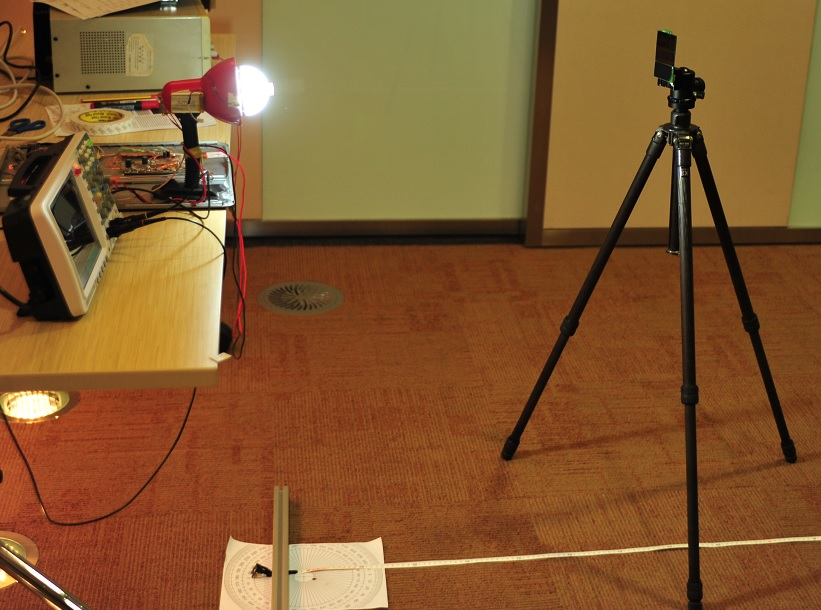
\includegraphics[width=0.7\columnwidth]{setup}
\vskip -0.05in
\caption{Evaluation testbed setup with a pair of ViReader and ViTag (For experiment with flash light reader, the lamp is replaced with flashlight reader).}
\label{fig:setup}
\vskip -0.05in
\end{figure}

%
%at various locations with different system settings. First we seek to validate it's point-to-point communication performance at varying data rates. Then we evaluate the security aspect of the system against a typical type of malicious behaviors, snifter.
%
%%\subsection{Evaluating the Communication Range}
%
%We evaluate the maximum communication distance between a \reader\ and a \vitag\ as a function of the LED illumination, solar cell size, retro-reflector size, tag orientation, angle of incidence at the reader and data rate. Maximum communication distance or range is defined as the longest distance at which the \vitag\ can respond to the \reader\. The \reader\ signals the successful receiving of a packet by a beep. We perform our experiments in three scenarios:
\paragraph{Testing Environments}
Being a VLC system specially designed for the indoor environments with lighting structure, we carried experiments in typical office environment, where the ambient light is maintained in a comfortable range around 300$lx$. The ViTag harvests energy not only from the \reader, but also from ambient light. On the other hand, the office environment comes with human movements and other disturbances that may affect communication. To give a sense of the environmental impact, we also test it in a dark chamber, as a baseline for comparison. In the dark chamber, the \reader LED is the sole light/energy source. 
%We note that the system performance is affected by the environment conditions. Therefore, we carry out evaluations in two representative environments: 
%\vskip 0.05in\noindent{\bf (1) Dark Chamber} Where the ViTag has the LED as the sole power source, a dark chamber also eliminates the environmental impact. This represents the controlled case which we use as the baseline. 
%\vskip 0.05in\noindent{\bf (2) Office ($\sim$300 Lux) } Offices are typical indoor places usually illuminated by artificial lighting systems. The ambient light is usually maintained within a comfort range around $300 Lux$. The ViTag harvests energy not only from the ViReader, but also from ambient light. However, the office environment comes with human movements and other disturbance that may affect communication.
                                                                                                                                                                                                                                                                                                                                                                                                                                                                                                                                                                                                                                                                                                                                                                                                                                                                                                                                                                                                                                                                                                                                                         
%\vskip 0.05in\noindent{\bf (3) Outdoor (day time)} Outdoor is another scenario where the ViTag actually gain energy from the sunlight \footnote{The outdoor night case is similar with the dark chamber which is thus not considered in our evaluations.}, which is different from artificial lighting. We perform our experiments on the sidewalk of a busy road. 
%\q{How would you do experiments for Night?}

\paragraph{Summary of Key Findings}
The key findings are highlighted as follows:
\begin{Itemize}
\item The experiments verify that we are able to get a \vitag\ to operate battery-free up to $2.4m$ away with lamp reader and $10.6m$ with flashlight reader (with package loss rate below $80\%$, or equivalent BER below $8.26\%$) and $0.5kbps$ data on the uplink. The system works for a wide range of \vitag orientations.
\item Reader-to-tag communication is resilient to eavesdropping. {\reader}s can only sense the ongoing communication in a visible range,  within a narrow the field of view of about $\pm 15\degree$.
\end{Itemize}

%\begin{figure*}[t]
%\minipage{0.32\textwidth}
%  \includegraphics[width=\textwidth]{../evaluation/PackageLostRate_Dark.eps}
%  \vspace{-2em}
%  \caption{Distance vs.\ packet loss rate in dark chamber and office room of 12W LED Lamp.}\label{fig:plr}
%\endminipage\hfill
%\minipage{0.32\textwidth}
%  \includegraphics[width=\textwidth]{../figures/angle_plr_100cm.eps}
%  \vspace{-2em}
%  \caption{Angle of incidence (irradiation) vs.\ packet loss rate.}\label{fig:readerAoI}
%\endminipage\hfill
%\minipage{0.32\textwidth}%
%  \includegraphics[width=\textwidth]{../figures/chargingtime_distance.eps}
%  \vspace{-2em}
%  \caption{Charging time vs.\ distance in dark chamber and office room.}\label{fig:charging_distance}
%\endminipage
%\end{figure*}


\subsection{Packet Loss Rate}\label{sec:plr}
%On the downlink, the transmitter is typically a powerful LED connected to the power line. Therefore, the bottleneck lies in the uplink. 
In this subsection, we focus on evaluating the packet loss rate (PLR) of the uplink tag-to-reader communication. For VLC, the received signal strength is mainly affected by three factors, i.e., the distance between ViTag and ViReader, the incidence angle, and the irradiation angle \cite{location3}.   

We first measure the impact of distance on PLR by varying the distance between ViReader and ViTag. We keep the ViReader perpendicular to the ViTag, i.e., $0\degree$ incidence or irradiation angles. To measure the PLR, the ViTag continuously sends packets for 20 minutes to ViReader with a constant rate. Each packet is consisted of $4 bytes$ ID data. We count the number of packets received successfully at ViReader. \figref{fig:plr} shows the resulting PLR versus distance. 

\begin{figure}[!ht]
\centering
\includegraphics[width=0.8\columnwidth]{../evaluation/PackageLostRate_Dark.eps}
\vskip -0.05in
\caption{Distance vs. PLR of 12W LED Lamp.}
\label{fig:plr}
\vskip -0.05in
\end{figure}

Figure ~\ref{fig:plr} shows that in a dark chamber, the PLR remains below $0.7\%$ in a distance up to $1.4m$. As the tag moves past $1.4m$, the PLR increases dramatically; Packets are barely received beyond $2.0m$. The drastic increase in PLR is because the energy obtained from the solar cell becomes insufficient in a long distance. In contrast, the PLR increases slower in the office environment thanks to the energy the ViTag harvests from the ambient light in addition to that from the ViReader. 

\begin{figure}[!ht]
\centering
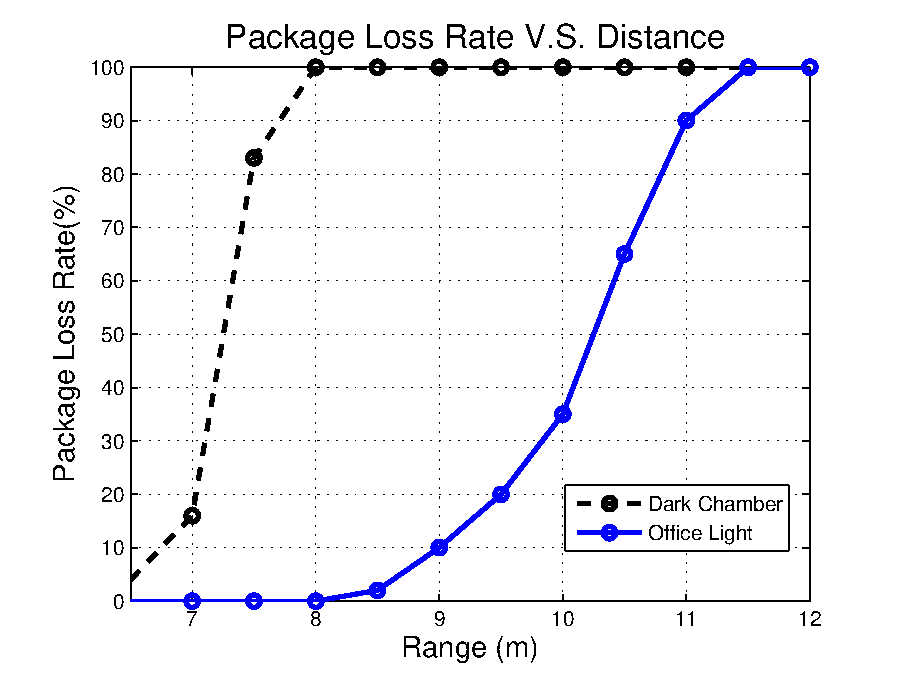
\includegraphics[width=0.8\columnwidth]{fig/PackageLostRate_flashlight.eps}
\vskip -0.05in
\caption{Distance vs. PLR of 3W flash light reader. X-axis starts from 6.5 meters}
\label{fig:plr_torch}
\vskip -0.05in
\end{figure}
Figure ~\ref{fig:plr_torch} presents the PLR as a function of the range for the 3W flash-light reader. The experiment shows that with the 3W flash-light reader, a much longer communication range can be reached. Specifically, in a dark chamber, instead of $1.4m$, the energy for receiving begins to drop significantly at $7.0m$, and nearly exhausts at $7.4m$. Under the situation with normal office lights, the system performs even better in terms of the communication range. The PLR remains at nearly 0 until the tag-reader distance reaches $8.5m$, and reaches $80\%$ at 10.6m. We can still receive package in a distance of $11.4m$.

%The dramatic increase in PLR is due to the threshold effect of the demodulator. We use a threshold during decoding the weak and noisy signal. In order to recover the drifting clock of the ViTag, we set a conservative threshold, and therefore lead to a sharp cut-off signal strength for successful decoding. 

\begin{figure}[!ht]
\centering
\includegraphics[width=0.8\columnwidth]{../figures/angle_plr_100cm.eps}
\vskip -0.05in
\caption{Angle of incidence (irradiation) vs.\ packet loss rate.}\label{fig:readerAoI}
\vskip -0.05in
\end{figure}

We then evaluate the PLR under different incidence or irradiation angles. Fix the distance between ViReader and the ViTag plane (the plane where the ViTag resides in 3D space), and move ViTag along the plane. In this setting, the incidence angle always equals the irradiation angle%\footnote{We note that these two angles are not identical in practice. However, our evaluation here represents the average case, and thus makes sense in reality.}. 
In our evaluation, we fixed the distance at $100$cm. The measured results are shown in \figref{fig:readerAoI}. We note that despite the seeming high PLR (\eg 80\%), for certain applications such as ID tag, we can still obtain the information after a few trials. This is similar to RFID systems. 



%\begin{figure}[tb!]
%\centering
%\includegraphics[width=0.45\columnwidth]{../figures/angle_plr_100cm.eps}
%\includegraphics[width=0.45\columnwidth]{../figures/angle_plr_200cm.eps}
%\vskip -0.05in
%\caption{\footnotesize{\bf Angle of incidence/irradiation at Reader V.S. PLR in a dark chamber and office room.} }
%\label{fig:readerAoI}
%\vskip -0.05in
%\end{figure}


%\paragraph{Maximum working range} We define the maximum communication range as the maximum distance between ViReader and ViTag such that ViReader is still able to decode the packet from ViTag. From Fig. \ref{fig:plr}, the maximum working range is thus 1.7 meters as discussed above.

\subsection{Response Time}\label{sec:bootstrap}
Response time accounts for the time from the ViReader issuing a query to receiving a response from the ViTag. Therefore, the response time consists of \textit{charging time}, downlink packet reception time, and uplink packet transmission time. Response time is a important metric for user experience. Generally, a response time below $100ms$ is thought to be negligible by human. In our system, due to the limitation of the LCD frequency, the uplink packet transmission time is slow, taking over $100ms$ to send a 32-bit ID. We envision faster LCD shutters in the future, and only focus on the charging time in the following.

\begin{figure}[!ht]
\centering
\includegraphics[width=0.8\columnwidth]{../figures/chargingtime_distance.eps}
\vskip -0.05in
\caption{Charging time vs.\ distance in dark chamber and office room.}\label{fig:charging_distance}
\vskip -0.05in
\end{figure}

If ViReader and ViTag are close enough, ViTag can quickly harvest enough energy to start conversation. Inversely, if the distance is long, ViTag needs a longer charging time before responding. We define the charging time as the time used to charge a \textbf{zero-initial-energy} ViTag. Charging time is affected by a number of factors like the solar cell size, ViTag energy consumption, and environment illumination level. %Among these, environment brightness has a significant impact on the charging time. For instance, in office area, the ViTag harvests energy from both the emitted light of ViReader and the existing indoor lighting system, thus reducing the charging time. 
As ViTag size is fixed, we only evaluate the impact from the environment illumination. 

First we evaluate the charging time as we vary the distance from $0.1m$ to $1.8m$, counting the time when the operation voltage raises from $10\%$ to $82.5\%$ (min operation voltage). The result is presented in Fig. \ref{fig:charging_distance}. We can see that, when the distance is small, the charging time in both cases are close. For instance, when the distance are $10$ or $20cm$, the charging time are around $50$ and $100ms$, respectively. The two curves begin to separate after around $0.6m$. The charging time in office environment grows slowly due to extra energy supply from the ambient light.


%\begin{figure}[tb!]
%\centering
%\includegraphics[width=0.7\columnwidth]{../figures/chargingtime_distance.eps} % {charging_time}
%\vskip -0.05in
%\caption{Charging time v.s. distance in a dark chamber and an office room. We show the raw measurements in markers and their polynomial fitting curves.}
%\label{fig:charging_distance}
%\vskip -0.05in
%\end{figure}
%

\begin{figure}[!ht]
\centering
\includegraphics[width=0.8\columnwidth] {../figures/angle_chargingtime.eps}
\vskip -0.05in
\caption{Charging time vs.\ incidence (irradiation) angles.}\label{fig:charging_angle}
\vskip -0.05in
\end{figure}

We note that the charging efficiency of the solar cell is also affected by the irradiation angle of the ViReader and also the incidence angle at the solar cell. For simplicity, we fix the distance between ViReader and the ViTag at $60$ and $120cm$, respectively, and observe charging time versus the incidence/irradiation angle shown in \figref{fig:charging_angle}. We indeed see increase in charging time with larger angles. However, the charging time grows slowly especially when the angle is small, e.g., below $30\degree$. This means the ViTag \fyi{tolerates flexible orientations} without experiencing serious performance degradation. In particular, we see much less sensitive reaction to the angles in office environment due to energy harvest from ambient light, which further highlights the benefit of using visible light as the power source.

%\begin{figure}[tb!]
%\centering
%\includegraphics[width=0.45\columnwidth]{../figures/chargingtime_angle_60cm.eps}
%\includegraphics[width=0.45\columnwidth]{../figures/chargingtime_angle_120cm.eps}
%\vskip -0.05in
%\caption{Charging time under different incidence/irradiation angles in a dark chamber and office room.} 
%\label{fig:charging_angle}
%\vskip -0.05in
%\end{figure}

In practice, ViTag can always harvest energy from ambient light (sunlight or artificial lighting systems) no matter whether a ViReader exists. Thus, the actual bootstrap can be instantaneous. This is a key difference from RFID/NFC tags where the operation energy can only be gained from a dedicated reader. 

\subsection{Channel Response}

\fyi{This subsection shows how energy of light signal attenuates against travelling distance along the visible channel. Here, the visible channel means the path along which the light signal traverses until it is received by the receiver of the reader, including the downlink, the retro-reflector, the LCD and the uplink.} For all backscatter systems, often times the energy of the signal received by the reader, which is reflected or backscattered by the tag, tends to be much weaker than the energy received by the tag, which poses a bottleneck for the system. %\fye{ According to the light reflection model of a standalone retro-reflector, the received energy attenuates proportionally to the square of the distance, which aligns with the theoretical model of the electromagnetic wave attenuation. Empirically, together with the lamp reader or the flashlight reader, however, the actual retro-reflector has a slightly diffusion angle, and the signal strength is affected by the non-linear auto-gain control (AGC) amplifier in the reader receiver. }
%
Thus, the energy efficiency is a crucial factor. To get an accurate picture of how energy diffuses as a function of the communication range, we measured the observed channel response for the lamp reader and flashlight reader. Fig.~\ref{fig:ChannelResponse} and Fig.~\ref{fig:ChannelResponse_flash} shows the energy calculated at the MCU, as the square of the output voltage. 
Note that the signal is captured and then measured by MCU, so it goes through Auto Gain Control(AGC) amplifier. 
From both figures, we see that when the tag is close to the LED, the signal is very strong and the AGC is effective. As a result, the portion of curves before AGC turned off goes down slowly. It actually almost completely suppresses the amplification when the signal is extremely strong (\ie, very close distance to the flashlight reader), as  shown in Fig.~\ref{fig:ChannelResponse_flash}. For both figures, after the point when AGC is turned off, \ie, always exerting maximum amplification, both curves attenuates at a rate square or cube of the distance.
\begin{figure}[!ht]
\centering
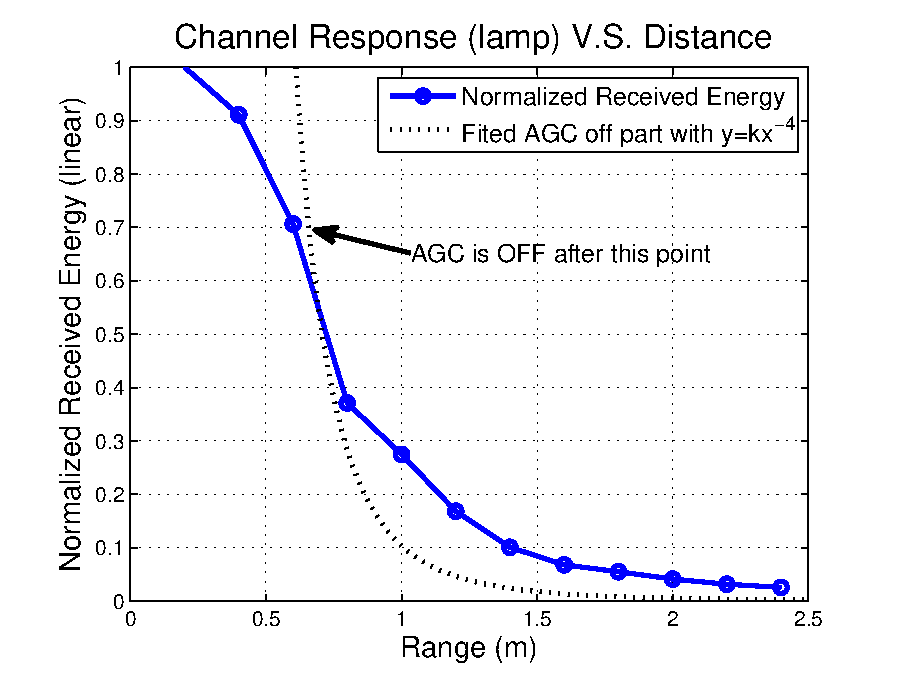
\includegraphics[width=0.77\columnwidth]{fig/ChannelResopnse_lamp.eps}
\vskip -0.05in
\caption{Channel responses of lamp reader}
\label{fig:ChannelResponse}
\vskip -0.05in
\end{figure}

\begin{figure}[!ht]
\centering
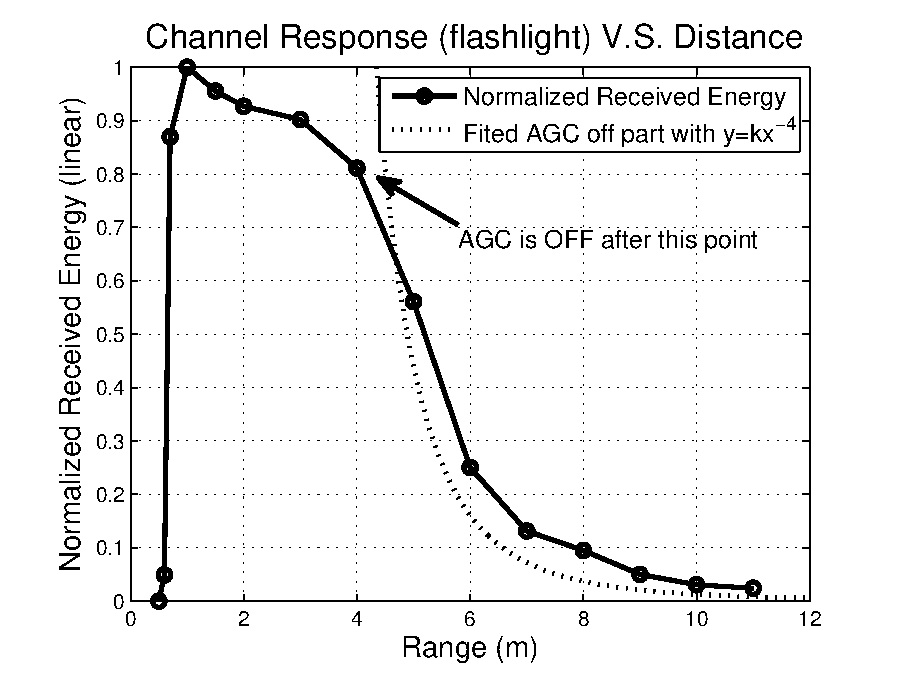
\includegraphics[width=0.77\columnwidth]{fig/ChannelResopnse_flashlight.eps}
\vskip -0.05in
\caption{Channel responses of flashlight reader}
\label{fig:ChannelResponse_flash}
\vskip -0.05in
\end{figure}


%

We note that, for a typical \textit{battery-free} backscatter system~\cite{abc1}, the wave front of the modulated backscattered signal received by reader from the tag attenuates proportionally to the power four of the communication range. A detailed formula can be found in paper~\cite{backscatterdeclay}.
%
As a comparison, we fit the part of the curve after AGC turns off to a negative quartic function, as the dotted line in Fig.~\ref{fig:ChannelResponse} and Fig.~\ref{fig:ChannelResponse_flash}. We can see that the negative quartic function attenuates much faster than our measurements. Thus, \retro achieves much better energy efficiency and can work at longer communication distance than typical battery-free backscatter systems for the same source emission power. This is perhaps due to the fact that \retro actually help concentrates lights from a scattering light source.%reflects light back along the same incoming direction with little scattering,}
% 


\subsection{Maximum Working Range}

We have so far evaluate both the PLR and energy harvesting. We then define the working range as the area within which the ViTag can harvest enough energy and talk with the ViReader with a chance above $20\%$, i.e., package loss rate is less than $80\%$. We measure the working range in office environment, and show the result in Fig. \ref{fig:ContinuesWorkingRange}. The working range in Fig. \ref{fig:ContinuesWorkingRange} is the area within the closed blue curve. With an upright orientation of the ViTag, the maximum working distance is up to $2.6m$. With ViReader perpendicular to the ViTag plane, the Field of View (FoV) is around $50\degree$. In our evaluation, we always make sure the same incidence angle and irradiation angle. Thus, the measured working range is conservative. In practice, if we orient the ViTag towards the ViReader, the FoV can be even larger. 

\begin{figure}[!ht]
\centering
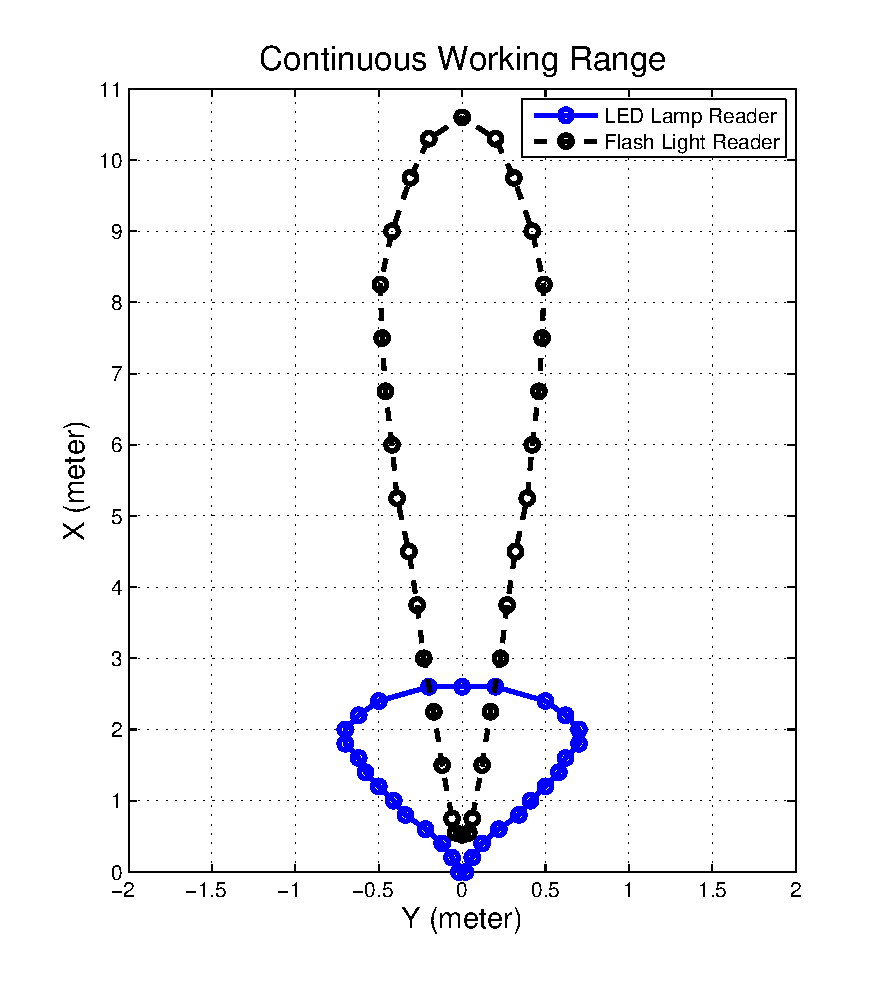
\includegraphics[width=0.7\columnwidth] {fig/ContinuesWorkingRange_flash.eps}
\vskip -0.05in
\caption{Working area measured in office environment. \fyi {Reader is located at (0,0).} }\label{fig:ContinuesWorkingRange}
\vskip -0.05in
\end{figure}

\fyi {As to flash-light reader, the max distance from the reader to the edge of the working area is 10.6m as shown in the figure. In our experiments, we can still receive packets at a maxim range of 11.3m. Note but, due to saturation, the flashlight reader can not work if the tag-reader distance is overly close, \eg., smaller than 0.5m, as show in \figref{fig:ContinuesWorkingRange}. This is due to the saturation of the sensors and amplification circuits. }

%\begin{figure}[tb!]
%\centering
%\includegraphics[width=0.8\columnwidth]{../figures/ContinuesWorkingRange.eps}
%\vskip -0.05in
%\caption{Working range measured in office environment.} 
%\label{fig:ContinuesWorkingRange}
%\vskip -0.05in
%\end{figure}

\subsection{Eavesdropping Range}\label{sec:secure}

Eavesdropping attacks in our system refer to a device secretly listening to the conversation between a ViTag and a ViReader. It is shown that eavesdropping is usually an early step of other attacks like man-in-the-middle attacks \cite{rfidsec1,rfidsec2}. One of the promising applications of \retro is using ViTag as a badge or payment card. Therefore, it is important that we protect the communication safety against eavesdropping attacks. 

\begin{figure}[!ht]
\centering
\includegraphics[width=0.7\columnwidth] {../figures/security_experiment_figure2.eps}
\vskip -0.05in
\caption{Signal detection radius of uplink. }\label{fig:security}
\vskip -0.05in
\end{figure}

A key feature of \retro compared with RFID/NFC is that the tag-to-reader communication is \textbf{directional}. Therefore, it is expected that a conversation from ViTag can only be detected within a narrow FoV. It is shown in \cite{eavesdrop2} that a sniffer can overhear NFC communication even over 1 meter away. In our evaluation, we place a ViReader and ViTag pair $0.6m$ apart from each other. The ViTag faces squarely to the ViReader, as shown in Fig. \ref{fig:security}. We use another reader as the attacker and measure the area where the attack can sniff the transmission from the ViTag. The area is plotted in Fig. \ref{fig:security}. 

%\begin{figure}[tb!]
%\centering
%\includegraphics[width=0.9\columnwidth]{../illustrations/security_experiment.eps}
%\vskip -0.05in
%\caption{\footnotesize{\bf Illumination v.s. Signal-Detectable Radius of Uplink.} The areas in both cases are spindle-shaped.}
%\label{fig:security}
%\vskip -0.05in
%\end{figure}

The signal can actually be detected quite far away as shown in Fig. \ref{fig:security}. As discussed in Fig. \ref{fig:plr}, 
The reason is that the retro-reflector is not perfect, it reflects the light back with a small diffusion angle. The intensity of light decays quickly with the angle. In our experiment, we use a sniffer that have {$100dBm$} gain(the same as our \reader), and the result shows the detectable area is nearly $2m$ in the back, excluding the shadow of the \reader.
%For This: the maximum range where the ViReader has a chance to receive packets from the ViTag is upto 2.6 meters. Therefore, the maximum signal-detectable distance from the ViReader is nearly 2 meters. 		
%Jinagtao: I'm wrong about that yesterday. Reader's Range have no relationship with the sniffer range. Because the angle is of much different between reader sensor and sniffer sensor when looking at the Tag. Thus the sniffer has less light intensity received.
However, the whole area resides within a small FoV of the ViTag, making it much easier for the user to discern the sniffer and can be blocked by a larger cover of \reader. Usually, the reader is fixed on the wall (e.g., a badge reader) which further reduces the signal-detectable area. 


%\q{If the maximum communication range is 2.6 meters, the round trip distance should be 2.6*2=5.2 meters. Then, the maximum signal-detectable distance is 5.2-0.6 = 4.6 meters. Is this what Jiangtao told me today??}

%\subsection{Evaluating \retro for Typical Applications}\label{sec:data_rate}
%In this section, we evaluate \retro in two typical applications. 
%
%The first application is using ViTag as a replacement of existing RFID/NFC cards, e.g., a badge. The use case is as follows. The user wears a credit card sized ViTag badge during work time. She needs to swipe her badge in front of a reader beside the door in order to get into a lab. Most existing badges are based on RFID which can only operate within a few centimeters from the reader. The range has to be short due to security considerations, which however make it less user friendly as the user has to explicitly do the badge swiping action. Basically, the communication between reader and RFID tag can easily be overheard in quite a large area even if the reader adopts a low transmission power \cite{guoliang's paper}. As shown in Section \ref{sec:secure}, the tag-to-reader transmission can only be heard within $\pm xx\degree$ ensuring the security even the distance is far. Therefore, with our ViTag badge, the user can actually remotely and automatically swipe the badge without explicit actions. 
%
%For the ViTag badge application, the key metric is the response time, i.e., how long the user needs to wait before the ViReader successfully decode the ViTag's ID. The waiting time depends on both the charging time and the BER. Generally, the longer the distance and the more slant the incidence/irradiation angles, the longer the waiting time. 

%\vskip 0.05in\noindent{\it Experiments.} We evaluate the communication range the system can achieve at a set of downlink and uplink data rates. The downlink rates tested include \hl{5kbps, 2kbps and 1kbps}, and the uplink rates tested include \hl{0.125kbps, 0.5kbps, 1kbps}. The downlink is set to \hl{5kbps} when evaluating the uplink, and the uplink is set to \hl{0.125kbps} when evaluating the downlink.
%
%\vskip 0.05in\noindent{\it Results.} Fig.~\ref{fig:datarate} (a) shows \hl{Shannon theorem} \hl{uplink data rate can be improved by using smaller voltage span for the LCD, which is enforced in the firmware instead of making modifications to the circuit}. Fig.~\ref{fig:datarate} (b) shows ...
%
%
%
%
%\begin{figure*}[!t]
%\vskip -0.1in
%\centering
%{\footnotesize
%\begin{tabular}{cc}
%\epsfig{file=../evaluation/DownRate_Range.eps, width=0.4\columnwidth} & \epsfig{file=../evaluation/UpRate_Range.eps, width=0.4\columnwidth}\\
%{(a) Evaluating Downlink}  & {(b) Evaluating Uplink}\\
%\end{tabular}
%}
%%\vskip -0.1in
%\caption{\footnotesize{\bf Data Rate V.S. Communication Range.} Blah Blah.}
%\label{fig:datarate}
%\vspace{-1em}
%\end{figure*}




%\subsubsection{Illumination v.s. BER}
%
%\begin{figure}[tb!]
%\centering
%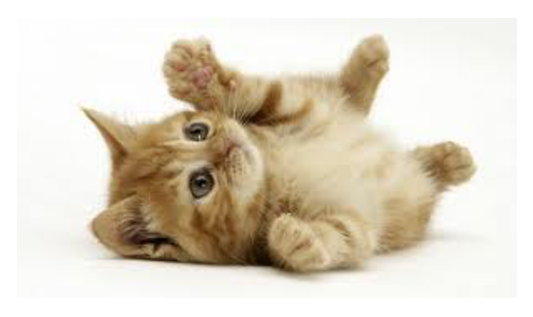
\includegraphics[width=0.7\columnwidth]{../figures/placeholder.eps}
%\vskip -0.05in
%\caption{\footnotesize{\bf Illumination v.s. BER.} blah blah.}
%\label{fig:ber1}
%\vskip -0.05in
%\end{figure}
%
%\subsubsection{Distance v.s. BER}
%
%\begin{figure}[tb!]
%\centering
%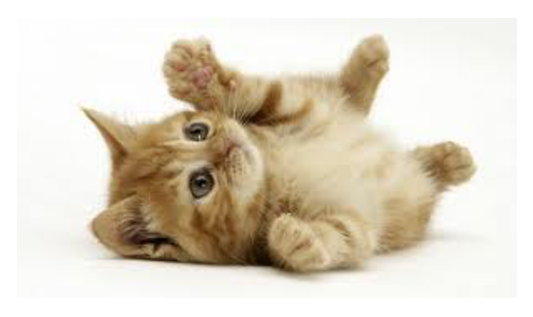
\includegraphics[width=0.7\columnwidth]{../figures/placeholder.eps}
%\vskip -0.05in
%\caption{\footnotesize{\bf Distance v.s. BER.} blah blah.}
%\label{fig:ber2}
%\vskip -0.05in
%\end{figure}

% \subsubsection{Retro-reflector Scattering}
% Due to surface defects, for example, not perfectly perpendicular micro-mirrors in the cubes, retro-reflectors render the reflected light scattered. We use \qm{a laser} that emits a nearly collimated beam to measure the scattering angle of the retro-reflector, with comparison to mirrors. Theoretically, suppose the mirror is not perfect, with an error angle $\Delta\theta$ that captures its surface defects. Suppose the retro-reflector has the same error angle that captures its surface defects on each of the three mirrors within a cube. 
% \q{What's this set of experiments aim at?}
% %\subsubsection{Illumination v.s. Charging time}


% \q{What kind of conclusion do we get from these experiments?}





% \subsubsection{Illumination v.s. Signal-Detectable Distance from the Tag}




% \begin{figure}[tb!]
% \centering
% 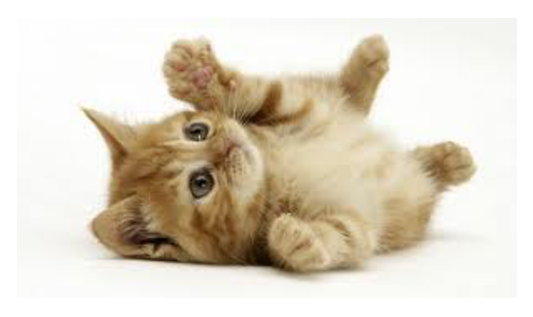
\includegraphics[width=0.7\columnwidth]{../figures/placeholder.eps}
% \vskip -0.05in
% \caption{\footnotesize{\bf Illumination v.s. Signal-Detectable Distance from the Tag.} blah blah.}
% \label{fig:security2}
% \vskip -0.05in
% \end{figure}



% \subsection{Evaluating Concurrent Transmissions}

% \subsubsection{\# of \vitag\/s Supported v.s. Communication Range}
% \hl{need another tag}
% \subsubsection{\# of \reader\/s Supported v.s. Communication Range}
% \hl{need another tag}



